\documentclass[11pt]{article}
%
% % Insert style guide
\usepackage{my_thesis}

% Specifiy the location of images to be used
\graphicspath{{figures/}}

%

\begin{document}
\title{\textsc{Surface waves extraction using transmission line Green functions in a multilayer environment with a 2D sheet}}

\date{\footnote{Last Modified: \currenttime, \today.}}

% Create title page
\maketitle

%\chapter{\uppercase{Surface waves extraction using transmission line Green functions in a multilayer environment with a 2D sheet}}



% \section{Abstract}

A semiconductor based multilayer structure in which an infinitesimally thin sheet representing a highly conductive two-dimensional electron gas (2DEG) is considered

\section{Theory}
\subsection{Derivation of Transmission line Green Function}

We follow the well-established approach of field computation for planar multilayered media \cite{michalski1997multilayered, michalski2005}, in which an equivalent transmission line network is set up for the structure. As shown in Fig. \ref{fig:TL_equivalent}a, it is assumed that the structure is unbounded in the lateral direction. The electric and magnetic fields are given by the Maxwell's equations,
\begin{subequations}
  \begin{align}
    \del\x{\v E} ={}& -j \O \u \v{H},
    \label{eq:E}\\
    \del\x{\v H} ={}& j \O \E \v{E} + \v{J}.
    \label{eq:H}
  \end{align}
  \label{eq:MaxE}%
\end{subequations}
%
For boundary-value problems displaying symmetry along the $z$ direction, it is desirable to decompose the $\v{\del}$ operator into two components, one $\dv{}{z}$ and the other a transverse (to z) operator, $\v{\del_t}$ \cite[p. 64]{felsen1994}. By taking the Fourier transform,
%
\begin{equation}
    \mathcal{F}[f(\v{r})] \equiv \ti{f}(\v{k_{\p}},z) = \infint \infint
    f(\v{r}) \e^{-\j \v{k_{\p}} \cdot \v{\p}} \diff{x} \diff{y}
    \label{eq:Fourier}
\end{equation}
%
the field computation is simplified by switching to the spectral frequency domain $\v {k_{\p}}$, which reduces the vector differential operator, $\v{\del}$ to $-\j k_x \v{\^{x}} - \j k_y \v{\^{y}} + \v{\^{z}}\dv{}{z}$. In \eqref{eq:Fourier}, the cylindrical coordinates are expressed as,
%
\begin{equation}
  \v{\p} = x\v{\^{x}} + y\v{\^{y}}, \quad \text{and} \quad
  \v{k_{\p}} = k_x\v{\^{x}} + k_y\v{\^{y}},
\end{equation}
%
and the notation $~$ above the terms indicates the Fourier transform with respect to the transverse coordinates and from here on, will be used to denote spectral quantities.

As stated earlier, it is advantageous to separate the fields in transverse and longitudinal coordinates since, as we shall shortly, the longitudinal part of the field can be completely expressed in terms of the transverse component. Appling the Fourier transform \eqref{eq:Fourier} on the Maxwell's equations \eqref{eq:MaxE}, we obtain:
%
\begin{subequations}
  \begin{align}
    \left(-\j \v{k_{\p}} + \v{\^{z}} \dv{}{z} \right)\x (\v{\ti{E}_t} + \v{\ti{E}_z})  ={}& -\j \O \u (\v{\ti{H}_t} + \v{\ti{H}_z}),
    \label{eq:FT_E}\\
    \left(-\j \v{k_{\p}} + \v{\^{z}} \dv{}{z} \right)\x (\v{\ti{H}_t} + \v{\ti{H}_z})  ={}& \j \O \E (\v{\ti{E}_t} + \v{\ti{E}_z}) -
    (\v{\ti{J}_t} + \v{\ti{J}_z}).
    \label{eq:FT_H}
  \end{align}
  \label{eq:FT_EH}%
\end{subequations}
%
The transverse and longitudinal components of the magnetic field can be separately expressed in \eqref{eq:FT_E} as,
%
\begin{subequations}
  \begin{align}
    -\j \v{k_{\p}} \x \v{\ti{E}_z} +
    \dv{}{z}\v{\^{z}} \x \v{\ti{E}_t} ={}&
    -\j \O \u \v{\ti{H}_t},
    \label{eq:FT_TH}\\
    -\j \v{k_{\p}} \x \v{\ti{E}_t} ={}&
    -\j \O \u \v{\ti{H}_z}.
    \label{eq:FT_LH}
  \end{align}
  \label{eq:FT_TLH}%
\end{subequations}
%
Using the vector cross product property \cite[p. 117]{fang2010},
%
\begin{equation}
  \v{A} \x \v{B} =\v{A} \cdot (\v{B} \x \v{\^{n}}) \, \v{\^{n}},
  \label{eq:vec}
\end{equation}
%
where the unit vector $\v{\^{n}}$ is normal to the plane containing vectors $\v{A}$ and $\v{B}$. A scalar form of the longitudinal component of the electric field is obtained by applying \eqref{eq:vec} on \eqref{eq:FT_LH},
%
\begin{equation}
   - \j \v{k_{\p}} \cdot (\v{\ti{E}_t} \x \v{\^{z}}) \, \v{\^{z}} =
   - \j \O \u \v{\ti{H}_z}
  \label{eq:FT_sLE}
\end{equation}
%
which can be written in the scalar form,
%
\begin{equation}
   - \j \ti{H}_z = \frac{- \j}{\O \u}
   \v{k_{\p}} \cdot (\v{\ti{E}_t} \x \v{\^{z}}).
  \label{eq:sLH}
\end{equation}
%
Now taking the vector cross product with unit vector $\v{\^{z}}$ on both sides of \eqref{eq:FT_TH}, the transverse electric field component is expressed as:
%
\begin{equation}
  \begin{split}
    \dv{\v{\ti{E}_t}}{z} ={}& -\j (\v{k_{\p}} \x \v{\ti{E}_z}) \x \v{\^{z}}
    -\j \O \u \v{\ti{H}_t} \x \v{\^{z}}\\
    ={}& -\j \v{k_{\p}} \ti{{E}_z} -\j \O \u \v{\ti{H}_t} \x \v{\^{z}}
  \end{split}
  \label{eq:dFT_ET}%
\end{equation}
%
where the BAC-CAB vector triple product identity, $(\v{A} \x \v{B})\x\v{C} = \v{B}(\v{A} \cdot \v{C}) - \v{C}(\v{A} \cdot \v{B})$ has been applied.

Following a similar procedure starting from (\ref{eq:FT_H}), we obtain the transverse magnetic field, and scalar longitudinal component of the electric field:
%
\begin{equation}
  \begin{split}
    \dv{\v{\ti{H}_t}}{z} ={}& -\j (\v{k_{\p}} \x \v{\ti{H}_z}) \x \v{\^{z}}
    + \j \O \E \v{\ti{E}_t} \x \v{\^{z}} +
    \v{\ti{J}_t} \x \v{\^{z}} \\
    ={}& -\j \v{k_{\p}} \ti{{H}_z} + \j \O \E \v{\ti{E}_t} \x \v{\^{z}}  +
    \v{\ti{J}_t} \x \v{\^{z}},
  \end{split}
  \label{eq:dFT_HT}%
\end{equation}
%
and,
\begin{equation}
  -\j \O \E \ti{E}_z =
  \j \v{k_{\p}} \cdot (\v{\ti{H}_t} \x \v{\^{z}}) + {\ti{J}_z}.
  \label{eq:sLE}
\end{equation}
%
Substituting \eqref{eq:sLE} in \eqref{eq:dFT_ET} gives us the transverse electric field component,
%
\begin{equation}
  \dv{\v{\ti{E}_t}}{z} =
  \frac{1}{j \O \E} \left( k^2 - \v{k_{\p}}\v{k_{\p}} \cdot \right) (\v{\ti{H}_t} \x \v{\^{z}}) + \v{k_{\p}} \frac{\ti{J}_z}{\O \E}.
  \label{eq:Et}
\end{equation}
%
Similarly, from \eqref{eq:sLH} and \eqref{eq:dFT_HT}, we obtain the transverse magnetic field,
%
\begin{equation}
  \dv{\v{\ti{H}_t}}{z} =
  \frac{1}{j \O \u} \left( k^2 - \v{k_{\p}}\v{k_{\p}} \cdot \right) (\v{\^{z}} \x \v{\ti{E}_t}) + \v{\ti{J}_t}
  \x \v{\^{z}}
  \label{eq:Ht}
\end{equation}
%
where $k = \O \sqrt{\u \E}$ in \eqref{eq:Et} and \eqref{eq:Ht} is the medium wavenumber.

The fields in \eqref{eq:Et} and  \eqref{eq:Ht} for arbitrarily aligned sources lie in the plane of a spectral coordinate system as illustrated in Fig. \ref{fig:SpCS}. A rotational transformation of the coordinate system such that the axes align with the vectors $\v{k_{\p}}, \v{\^z} \x \v{k_{\p}}$ \cite{itoh1980}, simplifies the procedure of finding the transmission line equivalent such that the TE and TM mode analysis can be performed separately. The coordinate transformation can be expressed as:
%
\begin{equation}
  \begin{bmatrix}
    \v{\^u} \\
    \v{\^v}
  \end{bmatrix}
  =
  \begin{bmatrix}
    \cos \phi & \sin \phi \\
    -\sin \phi & \cos \phi
  \end{bmatrix}
  \begin{bmatrix}
    \v{\^x} \\
    \v{\^y}
  \end{bmatrix}
  \label{eq:transformation}
\end{equation}
%
where $\phi$ is the angle between $\v{k_{\p}}$ and the positive x-axis. A transmission line analogue for the spectral fields, expressed in terms of modal voltages and currents can therefore, be written as \cite{kastner1988, michalski1997multilayered},
%
\begin{equation}
  \begin{bmatrix}
    \v{\ti{E}_t} \\
    \v{\ti{H}_t}
  \end{bmatrix}
  =
  \begin{bmatrix}
    V^{TM} & V^{TE} \\
    -I^{TE} & I^{TM}
  \end{bmatrix}
  \begin{bmatrix}
    \v{\^u} \\
    \v{\^v}
  \end{bmatrix}.
  \label{eq:EHVI}
\end{equation}
%
\begin{figure}[t!]
  \centering
  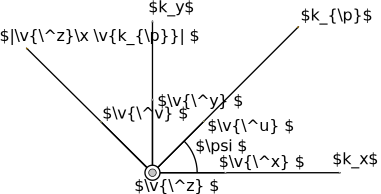
\includegraphics[width=.55\textwidth]{figures/xsystem.tikz}
  \caption{Coordinate System transformation in the spectral domain}
  \label{fig:SpCS}
\end{figure}

%
Using the results of \eqref{eq:EHVI} in \eqref{eq:Et} and noting that $\v{\^u} = \v{k_{\p}}/k_{\p}$, we get,
%
\begin{equation}
  \dv{\left(\v{\^u} \, V^{TM} + \v{\^v} \,V^{TE} \right)}{z} = \frac{1}{\j \O \E}\left( k^2 - \v{k_{\p}} \,\v{k_{\p}} \,\cdot \right) (\v{\^u}\, I^{TM} + \v{\^v} \, I^{TE}) + \v{\^u} \, \frac{k_{\p}}{\O \E} \ti{J}_z
  \label{eq:Vinuv}
\end{equation}
%
By separating the $\v{\^u}$ and $\v{\^v}$ components, we obtain the TM and TE equivalent voltage equations respectively,
%
\begin{subequations}
  \begin{align}
    \dv{V^{TM}}{z} ={}&
    \frac{1}{\j \O \E}\left( k^2 - k_{\p}^2 \right)I^{TM} + \frac{k_{\p}}{\O \E} \ti{J}_z,
    \label{eq:V_TM}\\
    \dv{V^{TE}}{z} ={}&
    \frac{k^2}{\j \O \E} I^{TE}.
    \label{eq:V_TE}
  \end{align}
  \label{eq:TL_Vs}%
\end{subequations}
%
Similarly, from \eqref{eq:EHVI} and \eqref{eq:Ht}, the equivalent current equations can be written as:
%
\begin{subequations}
  \begin{align}
    \dv{I^{TM}}{z} ={}&
    \frac{k^2}{\j \O \u} V^{TM} - \ti{J}_u,
    \label{eq:I_TM}\\
    \dv{I^{TE}}{z} ={}&
    \frac{-1}{\j \O \u}\left( k^2 - k_{\p}^2 \right)V^{TE} + \ti{J}_v.
    \label{eq:I_TE}
  \end{align}
  \label{eq:TL_Is}%
\end{subequations}
%
Equations \eqref{eq:TL_Vs}-\eqref{eq:TL_Is} can be conveniently written in a compact form as a set of Telegrapher's equations \cite[p. 1166]{michalski2005}:
%
\begin{subequations}
  \begin{align}
    \dv{V^{\alpha}}{z} ={}& -\j k_z Z^{\alpha}I^{\alpha} + v^{\alpha}
    \label{eq:TL_V}\\
    \dv{I^{\alpha}}{z} ={}& -\j k_z Y^{\alpha}V^{\alpha} + i^{\alpha}
    \label{eq:TL_I}
  \end{align}
  \label{eq:TLE}%
\end{subequations}
%
where the propagation constant in the transverse direction is,
%
\begin{equation}
  k_z = \sqrt{k^2 - k_{\p}^2}
  \label{eq:k_z}
\end{equation}
%
and the modal impedances are,
%
\begin{subequations}
  \begin{align}
    Z^{TM} = \frac{1}{Y^{TM}} = \frac{k_z}{\O \E},
    \label{eq:z_tm}\\
    Z^{TE} = \frac{1}{Y^{TE}} = \frac{\O \u}{k_z}.
    \label{eq:z_te}
  \end{align}
  \label{eq:Z}%
\end{subequations}
%
Assuming only electric sources existing in space, the corresponding TL sources, $v^{\alpha}$ and $i^{\alpha}$, where $\alpha$ is either TE or TM, are illustrated in \ref{fig:J_sources}. A horizontally oriented (x-directed) electric dipole is represented by a current source in an equivalent TM transmission line network. Likewise, the equivalent configuration of a vertical (y-directed) electric dipole is a TE network with a current source. A z-directed dipole corresponds to voltage source in a TM transmission line. For an arbitrarily directed source, the equivalent TL model consists of a superposition of the three representations.
%
\begin{figure}[h]
  \centering
  \subfloat[]{\centering
  \includegraphics[width=.55\textwidth]{figures/jx.tikz}
  \label{fig:jx_source}}  \newline
  \subfloat[]{ \centering
  \includegraphics[width=.55\textwidth]{figures/jy.tikz}
  \label{fig:jy_source}}  \newline \centering
  \subfloat[]{\centering
  \includegraphics[width=.55\textwidth]{figures/jz.tikz}
  \label{fig:jz_source}} \newline
  \caption{Electric Source Representation in a transmission line network}
  \label{fig:J_sources}
\end{figure}
%%%
%%%
%%%
%%%
\subsection{Equivalent TL network of semiconductor heterostructures}
%
In modern semiconductor devices such as a field-effect transistor, multiple layers of materials with slightly different dielectric properties and band-gap energies are epitaxially grown over each other. Of particular interest are the group III-V materials in which extra-ordinary electromagnetic interfacial phenomena is observed, mainly due to formation of a two-dimensional electron gas (2DEG) at the interface. To develop an understanding of the unusual properties of what are commonly called semiconductor heterostructures, we construct an equivalent transmission model of the layered structure using the theory discussed in the previous section.

An illustration of a multilayer setup with a heterostructure near the top of the transistor substrate, through which modern devices like the high electron mobility transistor operate, is shown in is shown in Fig. \ref{fig:TL_equivalent}a. Although a number of others layers exist underneath the heterostructure that are essential to the fabrication process in order to strengthen the epitaxial structure, only the top layers are conducive to an electric field. Moreover, since the widths of the layers in the heterostructure are much smaller than the rest of the layers in the substrate stack, we assume that the heterostructure is unbounded from the bottom.

The 2DEG which is only a few atoms wide in thickness, is a highly conductive region with an abundance of free electrons, which can be expresses in terms of a surface conductivity \cite{Burke2000},
%
\begin{equation}
  \sigma_s = \frac{N_s e^2 \tau}{m^{\ast}}\frac{1}{1 + \j \O \tau},
  \label{eq:sigma_s}
\end{equation}
%
where $N_s$ is the free electron concentration at the interface, $e$ is the electron charge, $m^{\ast}$ is the effective electron mass in the heterostructure, $\tau$ is the scattering time of electrons, and $\O$ is the angular frequency. For a wave propagating along the interface, the electron scattering time which is highly temperature dependent, determines the attenuation factor. At room temperature, the thermal vibrations of electrons result in a very small value of $\tau$ which is of the order of \SI{}{\ps} leading to a high-loss scenario. On the other hand, when the heterostructure is cooled to temperatures close to the boiling point of helium (\SI{4.2}{\kelvin}), thermal vibrations are effectively removed and the losses are consequently minimized.

In a transmission line analogue, a conductive sheet such as a 2DEG is represented by a shunt admittance as shown in Fig. \ref{fig:TL_equivalent}b In a high electron mobility transistor, when a voltage bias is applied across the source and drain terminals, a current starts to flow in the lateral direction in the 2DEG. Such a current source configuration corresponds to Fig. \ref{fig:jx_source}. Hence a TM-mode transmission line with a current source. The presence of a gate terminal above or below the interface allows the electron concentration to be modified with gate voltage control. Therefore, instead of an independent current source in the equivalent transmission line network, a voltage controlled source is used as shown in Fig. \ref{fig:TL_equivalent}.
%
\begin{figure}[t!]
  \centering
  \def\svgwidth{\linewidth}
  \input{figures/multilayers.pdf_tex}
  \caption{(a) Multilayer structure typically found in a high electron mobility transistor, (b) Equivalent transmission line network}
  \label{fig:TL_equivalent}
\end{figure}
%

We determine the dispersion relation in a 2DEG region which lies embedded in a semiconductor stack. As stated earlier, the active state of the transistor in which a current flows through the 2DEG corresponds to a TM-mode transmission line network. It must also be mentioned that a similar TL analogue can be obtained if the physical structure is excited by a TM-polarized plane wave. The dispersion relation can be written using the transverse resonance method that requires the total admittance as seen from the 2DEG (at z = 0) to be zero \cite{Gomez-Diaz2012},
%
\begin{equation}
  Y^{\uparrow}(z_0) + Y^{\downarrow}(z_0) + Y_{\sigma} = 0.
  \label{eq:dispersion}
\end{equation}
%
Here, $Y^{\uparrow}(z_0)$ and $Y^{\downarrow}(z_0)$ are the up- and down-looking TL admittances from the 2DEG located at $z = 0$ and $Y_{\sigma} = \sigma_s$ from \eqref{eq:sigma_s}.

A nontrivial solution of \eqref{eq:dispersion} in terms of the propagation constant $k_{\p}$ yields the surface wave modes of the structure in the complex k-plane.
%%%%%%%%%%
%%%%%%%%%%
%%%%%%%%%%
%%%%%%%%%%
%%%%%%%%%%
\section{Surface waves extraction technique}
%
We seek to solve \eqref{eq:def} in the complex z-plane to obtain the zeros, $z_k$ in a given search region $\mathbb{C}$. For a multilayer problem such as the one shown in Fig. \ref{fig:TL_equivalent}a, $f$ represents the dispersion relation \eqref{eq:dispersion} obtained from the characteristic equation of a Transmission Line Green function (TLGF), and $k_{\p}$ is replaced by $z$ for notational simplicity. Depending on the location of the zeros of the function $f$ in the complex plane, $z_k$'s correspond to the surface wave modes as well as the poles of the TLGF.
%
\begin{equation}
  f(k_{\p}) = 0
  \label{eq:def}
\end{equation}
%
Although the problem may at first appear to be a relatively simple root-search in which readily available and popular iterative algorithms like the Newton or Halley method can be applied, complication arises due to presence of complex-valued roots. Furthermore, the convergence of the aforementioned methods is highly subject to an initial guess that must lie close to the actual root. For a dispersion relation like in \eqref{eq:dispersion} that are defined as a transcendental equation, presence of singularities like poles and branch points particularly in the vicinity of an actual solution may leave an iterative method completely divergent or yet churn out a bogus and unreliable answer.

Argument principle method (APM) is a robust, complex root-finding algorithm in which convergence is guaranteed within a specified region without supplying any initial guess \cite{Delves1967c,Carpentier1982c,Botten1983,Kravanja2000c,Dellnitz2002c,Gillan2006c,Chen2017}. It requires the function to be analytic in the specified search region. A pictorial representation of this technique is shown in Fig. \ref{fig:zplane} where the roots inside a specified region $\Gamma$ in the complex plane are computed by approximating the given function with a polynomial. The number of zeros inside $\Gamma$ must not exceed a preallocated value $N_r$, otherwise the search region is reduced. Moreover, the function $f$ must be non-zero at the boundary of $\Gamma$. The following sections briefly describe each step of the method.
%
\begin{figure}[b!]
  \centering
  \def\svgwidth{.5\linewidth}
  \input{figures/zplane.pdf_tex}
  \caption{An illustration of a search region in the form of a rectangular controur $\Gamma$. If the zeros inside exceed a pre-allocated value, $\Gamma$ is split into smaller rectangles}
  \label{fig:zplane}
\end{figure}
%%
%%
%%
%%
\subsection{Counting the zeros}
%
To develop an efficient method of locating the zeros, we assume that the function $f$ is analytic, implying it is differentiable and free from any singularities. It is also required that $f$ is non-zero at the boundary, $\Gamma$ of the region $\mathbb{C}$. The search region is set as rectangular, mainly because of ease in programming it. The number of zeros, $N$ inside a region with a boundary $\Gamma$ can be found using the Cauchy's integral theorem \cite[pg. 71]{Krantz1999,Delves1967c},
%
\begin{equation}
  N = \frac{1}{2 \pi \j} \oint \limits_{\Gamma} \frac{f'(z)}{f(z)} \diff{z}
  \label{eq:cauchyth}
\end{equation}
%
where the integrand is a logarithmic derivative of the function. The analytical derivative of functions such as found in dispersion relations like \eqref{eq:dispersion} are seldom readily-available and it is generally cumbersome to compute. In this chapter, we use approximate the derivative by a finite difference formula,
%
\begin{equation}
  f'(z) = \frac{f(z + h) - f(z - h)}{2 h},
  \label{eq:FD}
\end{equation}
%
where $h \sim \sqrt{\epsilon_m}$ and $\epsilon_m = \SI{2.2204e-16}{}$ is the double-precison machine accuracy \cite[pg. 230]{press2007numerical}.

In addition to \eqref{eq:cauchyth}, a derivative-free form of the argument principle \cite{Carpentier1982c,Gillan2006c}, which may be preferred in certain cases is,
%
\begin{equation}
 N = \frac{1}{2 \pi} \oint \limits_{\Gamma} \diff {\{ \arg f(k_{\p})\}},
 \label{eq:numzeros}
\end{equation}
%
The value of both the integrals, i.e., \eqref{eq:cauchyth} and \eqref{eq:numzeros} is an integer which means that whenever a zero is encountered while performing the contour integration, the resulting integral is incremented by a factor of $2 \pi$. The contour integration in \eqref{eq:cauchyth} and \eqref{eq:numzeros} is computed in a counter-clockwise manner, using an adaptive Gauss-Konrod quadrature ({MATLAB}'s \emph{quadgk} routine) \cite{Shampine2008}. The contour can be conveniently set up using the `waypoints' parameter of the routine.
%%
%%
%%
%%
\subsection{Locating the zeros}
%
After predicting the number of zeros through \eqref{eq:numzeros} or \eqref{eq:cauchyth}, the function $f$ is then approximated by an associated \emph{formal orthogonal polynomial} (FOP), $\mathcal P$ of degree $N$, equal to the number of zeros. A necessary condition during approximation is that $\mathcal P$ must have the same roots, $z_k$ where $k = 1,2,...,N$ as $f$. Furthermore, as stated earlier $N$ must be less than $N_r$ to avoid a too-high order polynomial for which the root-finding procedure would be very slow.

The polynomial $\mathcal P$ can be represented in a Lagrange form:
%
\begin{equation}
  \begin{split}
    \mathcal{P}_N(z) ={}& \prod \limits_{k = 1}^N \left(z - z_k \right) \\
    ={}& z^N + \sigma_1 \, z^{N-1} + \sigma_2 \, z^{N-2} + \dots + \sigma_N.
  \end{split}
  \label{eq:poly}%
\end{equation}
%
To find the coefficients, \sigma_k, we consider a set of integrals that are termed as the \emph{Newton moments},
%
\begin{equation}
  s_k = \frac{1}{2 \pi \j} \oint \limits_{\Gamma} z^k frac{f'(z)}{f(z)} \diff{z}, \quad \text{where} \, k = 0,1,\dots, N
  \label{eq:s_k}
\end{equation}
%






For orthogonality, we require the inner product,
%
\begin{equation}
  \langle z^k{,} \mathcal{P}_N(z)\rangle = \frac{1}{2 \pi j} \oint \limits_{\Gamma} z^k \mathcal{P}_N(z) \frac{f'(z)}{f(z)} \dif z, \quad \mathrm{with}\quad k = 0,1,...,N-1
  \label{eq:fop}
\end{equation}
%
to be zero \cite{Kravanja2000c}. The polynomial approximation of the original function reduces the complexity of the problem as techniques for finding polynomial roots are robust and well-established. Before we proceed, for the sake of convenience in obtaining the required polynomial, we express $\mathcal{P}$ in an alternate summation notation:
%
\begin{equation}
  \mathcal{P}_N(z) = \sum \limits_{k = 0}^N \alpha_k z^k
  \label{eq:poly_sum}
\end{equation}
%
For a \emph{monic polynomial}, $\alpha_N = 1$, and $\alpha_k$ are the sums of products of zeros, $Z_k$.

Next we look at a sequence of integrals:
%
\begin{equation}
  s_k = \frac{1}{2 \pi j} \oint \limits_{\Gamma} z^k \frac{f'(z)}{f(z)} \dif z, \quad \mathrm{with}\quad k = 0,1,2,...
  \label{eq:sk}
\end{equation}
%
where the $s_k$'s are the \emph{Newton moments} and related to the unknown coefficients $\alpha_k$'s through the \emph{Newton identities}:
%
\begin{equation}
  \begin{aligned}
    s_1 + \alpha_1 ={}& 0 \\
    s_2 + s_1 \alpha_1 + 2 \alpha_2 ={}& 0 \\
    {\vdots}\\
    s_N + s_{N-1} \alpha_{1} + ... + s_1 \alpha_{N-1} + N \alpha_N ={}& 0
    \label{eq:newtid}
  \end{aligned}
\end{equation}
%
After using the Newton's identities to construct the associated polynomial, we set up an eigenvalue problem in terms of two Hankel matrices, $\mathbf H$ and $\mathbf H^<$ which is derived from the Companion matrix of the polynomial \cite{Gillan2006c}:
%
\begin{equation}
  \mathbf H =
  \begin{bmatrix}
    s_1 & s_2 & \cdots & s_k \\
    s_2 & s_3 & \cdots & s_{k+1} \\
    s_3 & s_4 & \cdots & s_{k+2} \\
    \vdots & \vdots & \ddots & \vdots \\
    s_k & s_{k+1} & \cdots & s_{2k} \\
  \end{bmatrix}
  \label{eq:Hmat}
\end{equation}
%
and
%
\begin{equation}
  \mathbf H^< =
  \begin{bmatrix}
    s_0 & s_1 & \cdots & s_{k-1} \\
    s_1 & s_2 & \cdots & s_{k} \\
    s_2 & s_3 & \cdots & s_{k+1} \\
    \vdots & \vdots & \ddots & \vdots \\
    s_{k-1} & s_{k} & \cdots & s_{2k-2} \\
  \end{bmatrix}
  \label{eq:Hmat<}
\end{equation}
%
The roots of the polynomial $\mathcal P$ are the generalized eigenvalues, $\lambda$ of the matrix pencil:
%
\begin{equation}
  \left( \mathbf H - \lambda \mathbf H^< \right) \mathbf x = 0
  \label{eq:evp}
\end{equation}
%
where the column vector $\mathbf{x}$ is the eigenvector.
%
\subsection{Refining the roots}
%
Approximating a function in a given contour with many zeros requires a higher-order polynomial that introduces computational problems. In addition, the integrals of the moments in \eqref{eq:sk} need to be evaluated with a higher-accuracy and the mapping between $s_k$ and $\alpha_k$ \eqref{eq:newtid} rseults in an ill-conditioned system. To overcome such pitfalls, a limit is enforced on the number of zeros in a given region. If the number of zeros exceeds a predetermined value $M$, the size of the search region is subdivided \cite{Delves1967c}. For problems pertinents to multilayer structures, a safe choice of $M$ is $3$.

The accuracy of the roots obtained from the eigenvalues,$\lambda_k$ of \eqref{eq:evp} is not always high. However, $\lambda_k$'s is an excellent inintial guess for any iterative root-search routine from the class of Householder's methods. We choose the \emph{Halley's} method having cubic convergence and the iteration formula:
%
\begin{equation}
  x_{n+1} = x_n - \frac {2 f(x_n) f'(x_n)} {2 {[f'(x_n)]}^2 - f(x_n) f''(x_n)}
  \label{eq:halley}
\end{equation}
%
with $f'(x)$ and $f''(x)$, the first and second order derivatives approximated by finite differences. In general the roots, $z_k$'s lie in the complex plane. The iteration \eqref{eq:halley} needs to be performed on both the real and imaginary parts simultaneously.

\subsection{Branch Cuts}

The TLGF for a multilayer possesses two types singularities in the complex plane. We are primarily interested in finding the pole singularities that correspond to guided modes. In addition, the branch point singularities correspond to the radiation modes. Branch points arise due to the propagation constant, $k_{zi}$ of the layers having semi-infinite dimensions. The dispersion relation shows an even dependence on $k_{zi}$ of the layers that have finite width, hence there is no corresponding branch point.   \cite[Section~5.3a]{felsen1994}. In order to satisfy Sommerfeld radiation condition that all fields must decay to zero at infinity, the proper sheet of the Riemann surface of the square-root function needs to be selected. This is accomplished by enforcing that the imaginary part of $k_{zi}$ that contributes a branch point, is negative everywhere.
%
\begin{equation}
  \Im (k_{zi}) < 0
  \label{eq:proper}
\end{equation}
%
%%%%%%%%%%%%%%%
%%%%%%%%%%%%%%%
%%%%%%%%%%%%%%%
\clearpage % Force Bibliography to the end of document on a new page.
% If using biber
% \printbibliography
% \addbibresource{zubairy}
% else bibtex
\bibliography{citations}
\bibliographystyle{ieeetran}

\end{document}
